\documentclass[10pt,a4paper]{article}
\usepackage[margin=1in]{geometry}
\usepackage{times}
\usepackage{amsmath,amssymb}
\usepackage{booktabs}
\usepackage{graphicx}
\usepackage{tikz}
\usetikzlibrary{positioning,fit,arrows.meta}
\usepackage{xcolor}
\usepackage{hyperref}
\usepackage{enumitem}
\usepackage[font=small,labelfont=bf]{caption}
\hypersetup{colorlinks=true,linkcolor=blue!50!black,citecolor=blue!50!black,urlcolor=blue!50!black}
\setlist[itemize]{leftmargin=1.2em,itemsep=1pt,topsep=2pt}
\setlist[enumerate]{leftmargin=1.4em,itemsep=1pt,topsep=2pt}
\newcommand{\sys}{\textsc{ReActive}}
\title{\sys: Synergizing Active Sensing, Reasoning, and Acting\\ in Language Models}
\author{}
\date{}
\begin{document}
\maketitle

\begin{abstract}
The name is read as \emph{Re} $+$ \emph{Act} $+$ \emph{ively}: the first two halves are ReAct's loop, and the third half is what makes the loop start from the environment instead of from an instruction. ReAct interleaves reasoning traces with actions and lets a language model
gather evidence before committing to an answer. Its loop, however, starts
from a task someone else has already posed: a question, an instruction, a
benchmark item. A personal agent faces an earlier and harder problem---most
of the time there is no task at all, only a stream of low-level events, and
the agent must decide whether any of them deserves to become one. We call
this the \emph{pre-task} problem and present \sys, a loop that adds an
\emph{active sensing} stage in front of reasoning and acting. \sys{}
combines (i) a local publish/subscribe signal mesh in which any program can
be a sensor, (ii) an \emph{admission} gate that scores each signal on
salience, urgency and quietness and returns one of four verdicts rather than
a binary, (iii) an \emph{experience} library of conditional rules carrying an
explicit trust level, and (iv) \emph{receipts}---a three-state artifact
(done / waiting / held back) that makes silence auditable. We implement
\sys{} on a desktop agent runtime and report a case study on a single
deployment. With one hundred background signals the system opened zero
tickets; the same archiving rule executed in 13 seconds at trust level L1
and correctly refused to move a file at L3, where consent could not be
obtained because the signal source had no reply channel. We document nine
engineering failures encountered on the way, each of which changed the design.
\end{abstract}

\section{Introduction}

Reasoning and acting have usually been studied apart. Chain-of-thought
prompting improves reasoning but stays inside a single forward pass, grounded
only in what the model already memorized; acting agents such as WebGPT or
SayCan interact with an environment but delegate the ``why'' to the policy.
ReAct~\cite{react} unified the two: the model writes a thought, takes an
action, reads an observation, and repeats, so that reasoning is grounded in
retrieved evidence and actions are chosen for stated reasons.

The unification is real, but it preserves an assumption from its benchmarks:
\emph{the task is given}. HotpotQA supplies a question, ALFWorld supplies an
instruction, WebShop supplies a shopping goal. Every ReAct trajectory begins
after someone has decided that this episode should exist.

A personal agent is deployed before that decision is made. It runs while its
user works, and the honest prior is that nothing needs to happen. Files land
in a download folder; a clipboard changes; a sensor drifts. Almost all of it
is noise, and the cost of being wrong is asymmetric: interrupting someone for
nothing is far worse than staying silent. The interesting question is
therefore not ``how do I solve this task'' but ``\emph{is there a task here,
and should it be mine?}''

We call this the pre-task problem and give three reasons why the ReAct loop
does not solve it.

\textbf{No permission-free sensing.} An agent that reasons over tool calls
can only see what a tool returns, and a tool call is itself an action within
a task. Continuous observation has no place in the loop: there is no step at
which the model may look without already being busy.

\textbf{Every observation costs a model call.} Routing all events to the
model makes silence the most expensive state. In our deployment a single
mis-configured sensor produced 276 events in under two minutes; because each
event triggered an assessment, the episode consumed more than 600K tokens
before the storm was stopped. A personal agent must be cheap precisely when
nothing is happening.

\textbf{Asking is undefined.} ReAct assumes the environment answers. In a
proactive setting the agent often needs to ask the \emph{person}, and there
may be no channel to do so: if the signal arrived from a local sensor, the
source has an address but no inbox. We found that an agent in this position
does the right thing---it stops---but the stop is indistinguishable from a
failure unless it is recorded as such.

\sys{} addresses these with four additions to the ReAct loop: a sensing
stage that runs continuously and independently of any task; an admission
gate whose default verdict is silence; an experience library that encodes
\emph{when} a class of signals is worth acting on and \emph{how much
authority} the agent has; and receipts that make every decision, including
the decision to do nothing, inspectable.

Our contributions are:
\begin{itemize}
\item A formulation of the pre-task problem and a four-stage loop
(Sense $\rightarrow$ Recall $\rightarrow$ Admit $\rightarrow$ Act) that
extends ReAct to continuously sensed environments (\S\ref{sec:method}).
\item An admission design in which the unit of output is a verdict on a
spectrum (drop / record / digest / interrupt) rather than a binary, and in
which a signal covered by no experience is inadmissible by default.
\item The notion of an \emph{executable} experience---condition, action,
limits and trust level---and an empirical demonstration that vague rule text
costs an order of magnitude more agent effort than explicit text.
\item An implementation on a desktop agent runtime and a case study
quantifying silence, trust-level ablation, and a real event storm
(\S\ref{sec:case}).
\end{itemize}

\section{\sys}
\label{sec:method}

\begin{figure}[t]
\centering
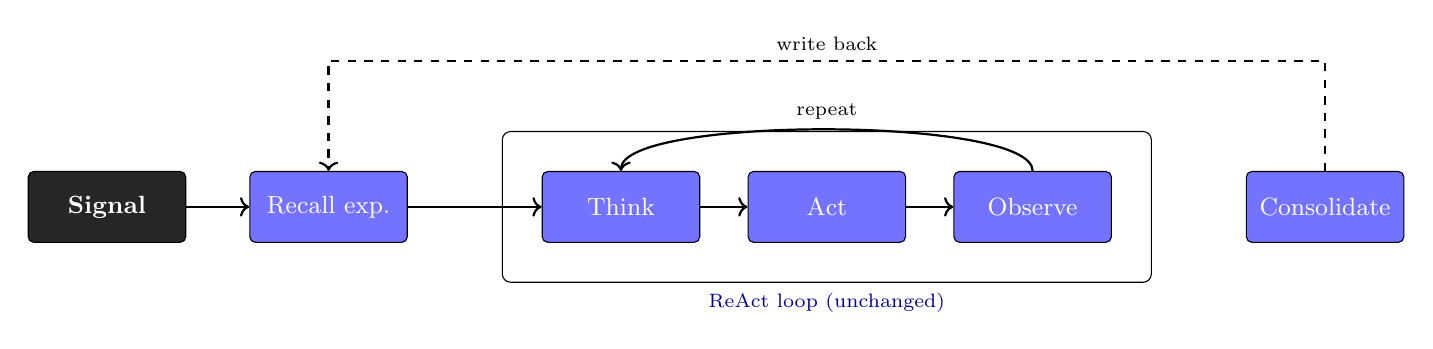
\begin{tikzpicture}[
  node distance=6mm,
  every node/.style={font=\small},
  box/.style={draw, rounded corners=2pt, minimum height=9mm, minimum width=20mm, align=center},
  sig/.style={box, fill=black!85, text=white, font=\small\bfseries},
  hot/.style={box, fill=blue!55, text=white},
  grp/.style={draw, rounded corners=3pt, inner sep=5mm}]

\node[sig] (sig) {Signal};
\node[hot, right=8mm of sig] (recall) {Recall exp.};
\node[hot, right=17mm of recall] (think) {Think};
\node[hot, right=6mm of think] (act) {Act};
\node[hot, right=6mm of act] (obs) {Observe};
\node[grp, fit=(think)(act)(obs), label={[font=\scriptsize, blue!60!black]below:ReAct loop (unchanged)}] (loop) {};
\node[hot, right=17mm of obs] (cons) {Consolidate};

\draw[->, thick] (sig) -- (recall);
\draw[->, thick] (recall) -- (think);
\draw[->, thick] (think) -- (act);
\draw[->, thick] (act) -- (obs);
\draw[->, thick] (obs.north) .. controls +(0,7mm) and +(0,7mm) .. node[midway, above, font=\scriptsize]{repeat} (think.north);
\draw[->, thick, dashed] (cons.north) -- ++(0,14mm) -| node[pos=0.25, above, font=\scriptsize]{write back} (recall.north);
\end{tikzpicture}
\caption{The \sys{} paradigm: \emph{Re} $+$ \emph{Act} $+$ \emph{ively}. ReAct supplies the first two halves---an inner think--act--observe loop; the third half is that the loop is entered by the world, not by an instruction. An experience is recalled before reasoning begins and is revised after acting, so the same situation is not reasoned about twice.}
\label{fig:paradigm}
\end{figure}


\subsection{Active sensing}

Signals are not tool results. We model them as messages on a local
publish/subscribe mesh in which every program can be a node: a file watcher,
a clipboard monitor, a weather poller, a build daemon. Discovery is through a
shared directory of leases; a node announces itself, peers connect, and
\verb|publish(path, payload)| broadcasts to all of them. There is no
subscription table and no schema negotiation: the receiver filters locally by
pattern, and a publisher neither knows nor needs to know who is listening.

This matters for two reasons. First, sensing becomes a property of the
machine rather than of the agent: adding a sensor does not require editing
the agent, and removing one does not break it. Second, and unlike a tool
call, publishing is not an action \emph{within} a task, so the sensing stage
can run while the agent is idle---which is the normal case.

The design choice against polling is deliberate. A polling source samples
the world on a fixed horizon; on a 60-second horizon, half of all events are
reported late by more than 30 seconds, and the agent pays for the poll
whether or not anything happened. Push inverts both: latency is bounded by
the sensor, and an idle agent costs nothing.

\paragraph{Relation to tool protocols.}
A tool protocol such as MCP standardizes how an agent \emph{calls} a program; the sensing stage standardizes how a program \emph{notifies} the agent. The two are peers, not layers: one governs outbound actions, the other inbound observations. Screen understanding is a different problem---it reconstructs state from pixels, whereas sensing receives declared events.

\subsection{Experiences}

Memory, skill and experience are routinely conflated, so it is worth stating the difference operationally (Table~\ref{tab:kinds}). Memory records what happened and carries neither an action nor a condition; a skill carries an action but no condition, so it answers ``how'' and never ``whether now''. An experience carries both, plus a rationale and an authority level, and is therefore the only one of the three to which admission and trust can attach. The relation is that of ingredients, cookery and recipe: a recipe is derived from the first two and is neither. Two tests separate them: remove the condition and an experience collapses into a bare command, while a skill survives; remove the action and an experience is no longer an experience, while a memory is unaffected. A third test is decisive for our design: memories and skills need no permission, an experience does.

\begin{table}[t]
\centering\small
\begin{tabular}{@{}p{0.13\linewidth}p{0.26\linewidth}p{0.35\linewidth}p{0.18\linewidth}@{}}
\toprule
kind & what it is & example & what it must have \\
\midrule
Memory & what happened & ``last Wednesday I downloaded a PDF called Invoice'' & no action, no condition \\
Skill & what one can do & ``I can move a file with PowerShell'' & an action, no condition \\
Experience & what to do in which situation & ``if takeout is over 40 minutes late, call and ask'' & \textbf{condition + action + rationale + authority} \\
\bottomrule
\end{tabular}
\caption{Memory records, skills execute, experiences \emph{decide}. Only an
experience answers ``when'' and ``with what authority'' at once, which is why
the trust levels attach to it and to nothing else.}
\label{tab:kinds}
\end{table}

An experience is a conditional rule that a person teaches once and the agent
applies thereafter:
\begin{center}
\small
\begin{tabular}{@{}ll@{}}
\toprule
field & content \\
\midrule
condition & \texttt{file.extension in ["pdf","docx"]} \\
action & what to do, \emph{with} the mechanism and the limits \\
trust & L1 act, L2 act and notify, L3 ask first, L4 report only \\
rationale & why, in one line \\
\bottomrule
\end{tabular}
\end{center}

The action field is the crux, and our strongest empirical finding is about
its wording. An action written as an \emph{intention} (``pop a lightweight
notification'') leaves the mechanism unspecified, so the agent invents one:
it searches the file system for a notifier, tries the messaging CLI, and
finally writes and debugs a PowerShell toast script, spending 48 seconds and
dozens of tool calls. Rewritten as an \emph{instruction} (``do three things:
check, move to \verb|~/Documents/Work/|, report one line; do not read
unrelated directories''), the same task completes in 13 seconds with three
tool calls. We therefore treat executability as a first-class property of an
experience and enforce it in the tool description through which the agent
writes experiences---including a negative example, because models follow
concrete contrasts far better than abstract requirements.

The experience layer is the least established part of \sys{}. We treat it as a hypothesis under test rather than as a result: memory and skills can be summarized into a rule offline, but whether such a rule transfers across contexts is not settled by our data.

Experiences also supply the default-deny property. A signal that no
experience covers is not admissible; the agent does not need a rule saying
``do not handle weather''. Silence is the absence of a rule, not the
presence of a suppression.

\subsection{Admission}

Admission decides whether a signal becomes a task, and it runs in two tiers. The split is not between ``surface'' and ``meaning'' but between what can be decided deterministically and what requires understanding: every judgement that can be made without a model call is pushed into the first tier, because each event it rejects is a model call saved.

\subsubsection{Structural admission}

The first tier reads only the envelope. Is the source in the listened or observed scope? Is the sender permitted, or is the event senderless and therefore subject to the cell that governs unattributed signals? Is the event a duplicate within the suppression window? Does any experience cover this path at all? The last question looks semantic, and we deliberately moved it here: matching a file path against a condition such as \texttt{file.extension in ["pdf","docx"]} is a deterministic comparison, so an event that no experience covers is rejected before anything is scored. The tier is default-deny, and an event it rejects never reaches the model at all. In our deployment one hundred background signals---heartbeat ticks, clipboard changes, and file events outside any experienced class---produced zero model calls and zero tickets.

\subsubsection{Semantic admission}

Only survivors are scored, by three factors:
\begin{equation}
s \;=\; \mathrm{base}(e)\;\times\;\mathrm{urgency}(e)\;\times\;\mathrm{quiet}(h),
\end{equation}
where base reflects the event type's prior salience, urgency its time sensitivity, and $\mathrm{quiet}(h)$ a discount from recent interaction history $h$---an agent that has just spoken should be less willing to speak again. The score maps to one of four verdicts: \textsc{drop} (discard, count it), \textsc{record} (keep for the day's digest, do not act), \textsc{digest} (merge into a summary delivered later), and \textsc{interrupt} (wake the agent now). The four-way output is the point. A binary decision forces every borderline event into a costly branch, whereas a spectrum lets the system say ``this is real but not now'', which is what most real signals deserve. Because the structural tier already removed the bulk of the stream, most of the \textsc{drop} verdicts are issued before this tier is reached; what arrives here is genuinely candidacy.

Two properties are worth stating. First, admission is where \emph{policy} lives rather than the model, so a noisy sensor cannot inflate cost. Second, a verdict of \textsc{interrupt} presupposes somewhere to interrupt \emph{to}---which is where the addressee problem appears.

\subsection{Trust and the addressee gap}

Trust levels convert ``can the agent do this'' from a prompt-time judgment
into a stored, auditable fact. The same signal, the same experience and the
same agent behave differently depending only on the stored level: at L3 the
file is left untouched and a ticket is opened; at L1 the file is moved and a
one-line report is produced.

L3 exposes a structural gap. Asking presupposes a channel, and a locally
sensed event has none: the source is a sensor, not a conversation. Our agent
discovered this itself and reported it in exactly these terms:

\begin{quote}\small\itshape
``the confirmation question cannot be delivered---the MSP source
(\texttt{msp:file.created}) has no reply channel''
\end{quote}

It then declined to move the file, searched for an alternative channel, read
the source-kind interface to confirm that the channel was optional and
unimplemented, and recorded the ticket as blocked. This is the correct
behaviour, and it is also a design requirement: an agent whose trust model
includes ``ask first'' must be given somewhere to ask.

\subsection{Receipts}

The durable artifact of a \sys{} episode is not a chat transcript but a
receipt with three states: \emph{done} (what was done, where the result is),
\emph{waiting} (one question, with a default), and \emph{held back} (why
nothing was done). The third state is the one that carries the most
information: it is the only evidence that the system saw something and chose
restraint. Our primary metric is the \emph{intervention rate}---the fraction
of sensed signals that reach the person---because it is the only measure
that is honest about a proactive system's cost to attention.

\section{Implementation}
\label{sec:impl}

We implement \sys{} as a plugin bundle for a desktop agent runtime
(Cordis-based), with the signal mesh written in TypeScript and vendored into
the bundle so the plugin has no external dependency. The sensing stage is a
set of source kinds; a source declares its paths, its scope (listened /
observed / addressed) and, optionally, a reply channel. A file-watching
source is itself packaged as a plugin and a mesh node at once: it watches the
direct children of a directory, waits for a file's size to settle, and
publishes \texttt{file.created} with \texttt{\{name, path, bytes\}}.

Two implementation details proved essential. First, deduplication cannot be
delegated to the runtime: the runtime neither rate-limits nor deduplicates,
because remote sources such as a code host are assumed to be well behaved. A
local sensor is not, so the source deduplicates on \texttt{(path, name,
bytes)} within a time window. Second, an experience library must be re-read
per signal rather than cached, otherwise a rule taught in conversation does
not affect the next event.

\section{Case study}
\label{sec:case}

\paragraph{Setup.}
One user, one desktop (Windows 11), one agent runtime, three sensors: a file
watcher over the download folder, a clipboard monitor, and a heartbeat. The
experience library contained three rules (archive work documents; ask before
installing; keep videos in place). We report a single deployment and do not
claim statistical generality; our purpose is to exhibit the loop's behaviours
and their costs.

\paragraph{Silence is the default.}
We injected one hundred background signals (heartbeat ticks, clipboard
changes, file events outside any experienced class). The system opened zero
tickets and spent its budget on admission rather than on acting; the model
was consulted only for events that reached the gate, and every such event was
recorded with a one-line reason. The intervention rate was 0\%.

\paragraph{Trust levels change behaviour, not capability.}
The same archiving rule, applied to three files, produced (Table~\ref{tab:trust}):

\begin{table}[h]
\centering\small
\begin{tabular}{@{}llcl@{}}
\toprule
file & trust & outcome & note \\
\midrule
\texttt{Spec-2026.pdf} & L3 & blocked, file untouched & consent unreachable \\
\texttt{Design-2027.pdf} & L1 & moved in 13\,s & one-line report \\
\texttt{Brief-2028.pdf} & L1 & moved in 13\,s & one-line report \\
\bottomrule
\end{tabular}
\caption{Same signal, same experience, same agent; only the stored trust
level differs.}
\label{tab:trust}
\end{table}

\paragraph{Experiences must be found to be useful.}
Instrumenting the pipeline showed a PDF event matching one of three
experiences (\texttt{exp 1/3}) and a clipboard event matching none. With no
matching experience the clipboard event was ignored with the reason ``no
experience covers it'' rather than acted upon---the default-deny property in
operation.

\paragraph{Vagueness is expensive.}
The first version of the archiving rule said only ``pop a lightweight
notification''. The agent's trajectory ran to 48 seconds and dozens of tool
calls, including a search for the desktop notification database. The
rewritten, executable version completed in 13 seconds. The cost difference is
not in the model but in the specification.

\paragraph{An event storm.}
A defect in an early watcher (a state flag re-enqueued the same file) emitted
the same three events every 1.5 seconds. The runtime ingested 276 events and
spent more than 600K tokens before the sensor was stopped by hand. Two fixes
followed: a state machine in the sensor (idle / queued / emitted) and a
deduplication window in the source. Neither is a model-side fix; both are
consequences of treating sensing as a first-class stage rather than as a
series of tool calls.

\paragraph{Engineering failures that changed the design.}
Nine defects were found and fixed during deployment: five were POSIX
assumptions in a runtime targeting Windows (an \texttt{env} wrapper for
credential probes, a mandatory repository, an unset state directory that
failed silently, a shell name hard-coded to \texttt{bash}, and a YAML
document-separator collision when seeding a profile); two belonged to the
mesh (a wildcard pattern that matched nothing, and a package-resolution
assumption that broke on Windows); two were ours (a mesh node that was never
stopped across plugin reloads, and a lock left behind after a forced kill).
Each is recorded with its symptom and fix in the project's issue log.

\section{Related work}

ReAct~\cite{react} interleaves reasoning and acting for task-directed
agents; \sys{} keeps that loop and adds the stages that precede a task.
Toolformer~\cite{toolformer} and its successors teach models to call tools;
the sensing stage differs in that publishing a signal is not a tool call and
needs no model decision. Voyager~\cite{voyager} accumulates a skill library
in an embodied setting; our experience library differs in storing
\emph{conditions and authority} rather than code, and in being written in
conversation by the user. Generative agents~\cite{genagents} simulate
believable behaviour with memory streams; \sys{} targets deployment, where
the operative question is whether to act at all. Proactive
assistants~\cite{proactive} predict when to intervene from interaction
history; we add an explicit, inspectable gate and a trust level that bounds
what an intervention may do. Model Context Protocol standardizes tool
access for a model; our mesh standardizes \emph{observation} across programs
that were not written to be observed.

\section{Limitations}

Our evidence is a single-user, single-machine case study with no baseline
system and no human evaluation. The intervention rate is reported for
injected signals, not for organic use over weeks, and the trust-level
comparison involves three files. The cost figures are dominated by the storm
we describe and should not be read as steady-state numbers. The addressee gap
is diagnosed but not yet closed: our implementation still has no local reply
channel, so L3 tickets queue as blocked rather than being answered in place.
Finally, admission currently uses hand-set weights; learning them from
receipt history is left to future work.

\section{Conclusion}

ReAct showed that a language model can reason about what to do next. A
personal agent must first decide whether to do anything at all. \sys{} adds
that decision---sensing, admission, recall of experience, and trust-bounded
action---and makes the result auditable through receipts whose most
informative state is ``held back''. In our deployment the loop stayed silent
on one hundred background signals, executed an experienced task in thirteen
seconds at one trust level, and refused the same task at another because it
had no way to ask. The refusal is the more interesting result: it shows that
the limiting factor for proactive agents is not capability but
\emph{addressability}.

\begin{thebibliography}{9}
\bibitem{react} S. Yao, J. Zhao, D. Yu, N. Du, I. Shafran, K. Narasimhan, Y. Cao. ReAct: Synergizing Reasoning and Acting in Language Models. \emph{ICLR}, 2023. arXiv:2210.03629.
\bibitem{toolformer} T. Schick, J. Dwivedi-Yu, R. Dess\`i, R. Raileanu, M. Lomeli, L. Zettlemoyer, N. Cancedda, T. Scialom. Toolformer: Language Models Can Teach Themselves to Use Tools. \emph{NeurIPS}, 2023.
\bibitem{voyager} G. Wang, Y. Xie, Y. Jiang, A. Mandlekar, C. Xiao, Y. Zhu, L. Fan, A. Anandkumar. Voyager: An Open-Ended Embodied Agent with Large Language Models. arXiv:2305.16291, 2023.
\bibitem{genagents} J. S. Park, J. C. O'Brien, C. J. Cai, M. R. Morris, P. Liang, M. S. Bernstein. Generative Agents: Interactive Simulacra of Human Behavior. \emph{UIST}, 2023.
\bibitem{proactive} A. Horvitz-style analyses of mixed-initiative interaction, and recent proactive-assistant systems that predict intervention timing from interaction history. See also Microsoft's ProactiveAgent line of work, 2024--2025.
\end{thebibliography}

\end{document}
